\chapter{Introducción específica} % Main chapter title

\label{Chapter2}

%----------------------------------------------------------------------------------------
%	SECTION 1
%----------------------------------------------------------------------------------------
En este capítulo se describen las tecnologías, herramientas y protocolos utilizados para la realización del trabajo.

\section{Protocolos de comunicación}
\label{sec:Protocolos de comunicación}
A continuación se describen los principales protocolos empleados en el trabajo. En la figura \ref{fig:IotProtocols} se observa su posicionamiento en la pila de protocolos para IoT.

\begin{figure}[h]
	\centering
	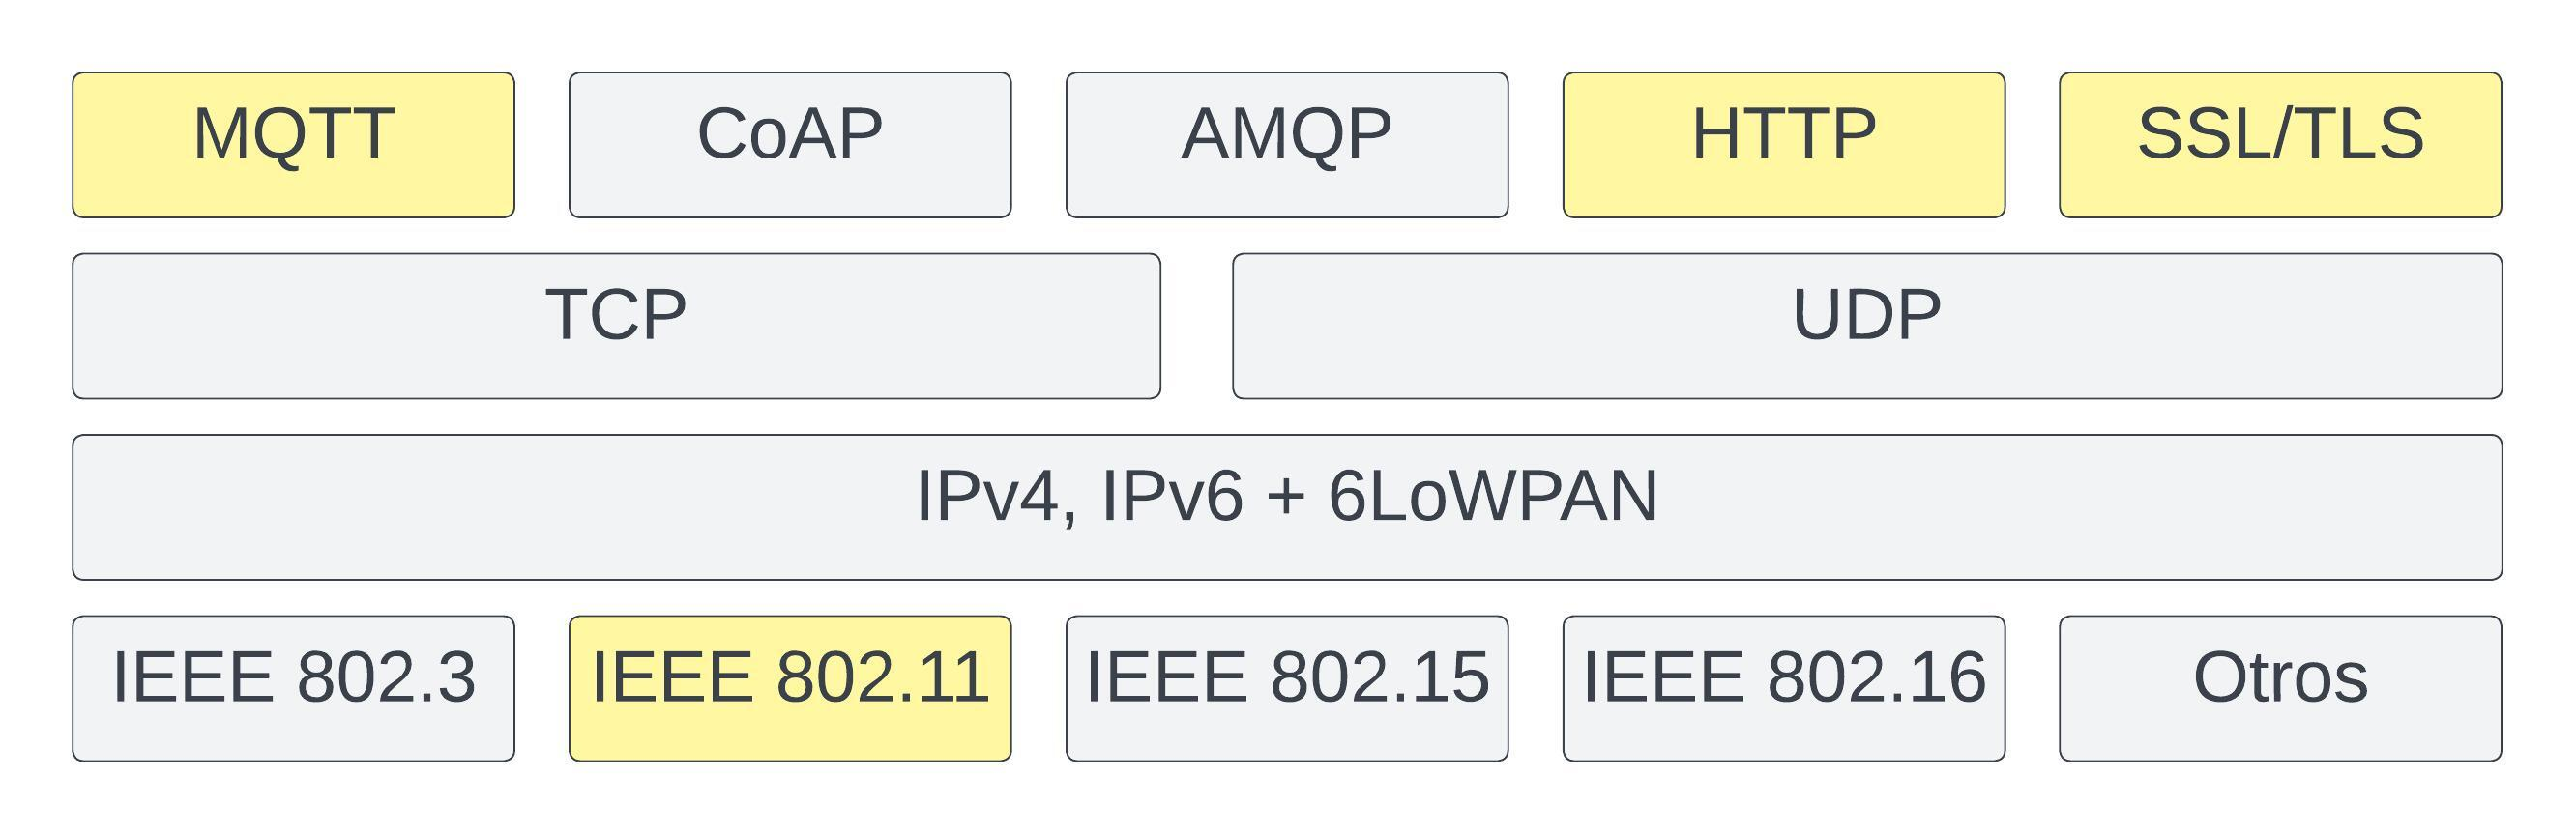
\includegraphics[width=0.75\textwidth]{./Figures/protocols.jpeg}
	\caption[Pila de protocolos para IoT.]{Pila de protocolos para IoT\protect\footnotemark.}
	\label{fig:IotProtocols}
	\footnotetext{Gráfico creado en base a una imagen tomada de: \citep{8088251}.}
\end{figure}


\subsection{Tecnologías Wi-Fi}
\label{sec:Tecnologías Wi-Fi}
El estándar IEEE 802.11 para redes inalámbricas de área local (WLAN) es conocido comercialmente como Wi-Fi. Este estándar presenta dos modos de operación \citep{wifi}
\begin{itemize}
\item Infraestructura: uno o máa \textit{access points} (AP) actúan como puente entre la red cableada y la red inalámbrica. Todas las comunicaciones entre los dispositivos conectados a la red, se realizan a través de los APs. 
\item Ad-hoc: cada nodo puede realizar una conexión directa con otro, sin necesidad de un AP central. Para lograr esto, los nodos se organizan en una red donde todos son capaces de enrutar los paquetes.  
\end{itemize}

\subsection{Protocolo MQTT}
\label{sec:Protocolo MQTT}
MQTT es uno de los protocolos de comunicación M2M (\textit{Machine to Machine}) más antiguos, introducido en 1999. Fue desarrollado por Andy Stanford-Clark de IBM y Areln Nipper de Arcom Control Systems Ltd\citep{8088251}. Es un protocolo de mensajería basado en el modelo de publicación/suscripción diseñado especialmente para operar en dispositivos de bajo costo y consumo de energía, sobre redes de capacidades limitadas \citep{4554519}.

\section{Componentes de hardware utilizado}
\label{sec:Hardware utilizado}

\section{Tecnologías de software aplicadas}
\label{sec:Software aplicado}

\section{Requerimientos}
\label{sec:Requerimientos}

